\subsection{Arquitectura  del servidor}

\begin{figure}[H]
\centerline{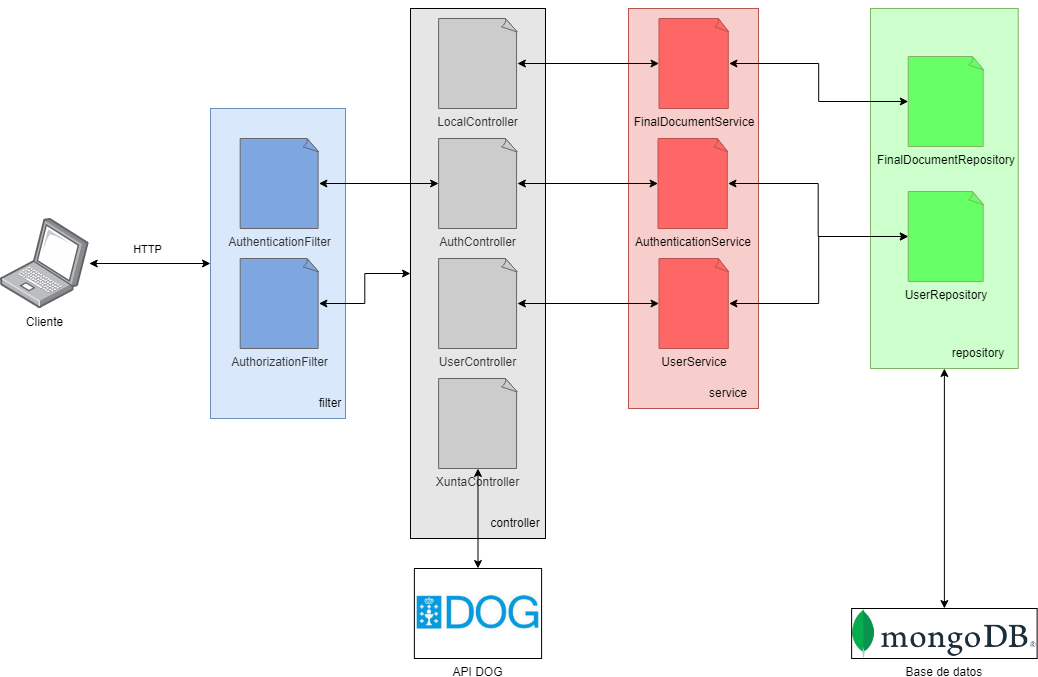
\includegraphics[width=15cm]{figuras/diseño/FicherosServidor.png}}
\caption{Arquitectura del servidor.}
\label{enlaceArquitecturaServidor}
\end{figure}

La arquitectura del servidor se muestra en la \hyperref[enlaceArquitecturaServidor]{Figura 3.2}, y en ella se pueden ver a simple vista los diferentes componentes que la forman.
\\

El usuario realiza desde el cliente las llamadas a la API mediante solicitudes HTTP (ya sean GET, POST, ...), de las que posteriormente obtendrá una respuesta. Una vez llegan las solicitudes al servidor, se hacen pasar por los filtros ({\it filter}). Encontramos por un lado el componente {\bf AuthenticationFilter}, que se encarga de gestionar el inicio de sesión, y, por otra parte, {\bf AuthorizationFilter}, que comprueba los permisos del usuario, así como si el token de la sesión es válido.
\\

Una vez pasan los filtros, la información se redirige hacia los controladores ({\it controller}). Estos controladores redirigen las llamadas a los servicios necesarios ({\it service}), que es donde se implementa la lógica de negocio en la aplicación. Por último, los servidores invocan a los métodos de los repositorios ({\it repository}), que son los que se encargan del acceso y almacenamiento en la base de datos.
\\

Teniendo en cuenta la división en componentes realizada, las funcionalidades de los distintos controladores, servicios y repositorios se pueden resumir en:
\begin{itemize}
    \item {\bf LocalController, FinalDocumentService y FinalDocumentRepository}: se encargan de gestionar las operaciones relacionadas con las leyes almacenadas en la base de datos de la aplicación. Desde LocalController se llama a los servicios necesarios de FinalDocumentService, el cual finalmente llama a FinalDocumentRepository para que maneje los datos de las leyes en la base de datos.
    \item {\bf UserController, UserService y UserRepository}: se encargan de gestionar las operaciones relacionadas con los usuarios, los cuales se almacenan en la base de datos de la aplicación. Desde UserController se llama a los servicios necesarios de UserService, el cual finalmente llama a UserRepository para que maneje los datos de los usuarios en la base de datos.
    \item {\bf AuthController, AuthenticationService y AuthenticationFilter}: se encargan de gestionar las operaciones relacionadas con aspectos de seguridad respecto a los usuarios, como el inicio de sesión. Acceden también a los usuarios almacenados en la base de datos local. Desde AuthController se llama a los servicios necesarios de AuthenticationService, el cual finalmente llama a AuthenticationFilter para que maneje los datos de las leyes en la base de datos. En este caso es necesario utilizar el filtro de AuthenticationFilter, pues se encarga del inicio de sesión.
    \item {\bf XuntaController}: se encarga de gestionar las llamadas a la API del DOG. De aquí el controlador XuntaController obtiene las diferentes leyes encontradas en el DOG.
\end{itemize}

\subsubsection{Listado de servicios}

Como se ha mencionado anteriormente, el servidor sigue una arquitectura basada en servicios REST, los cuales permiten el acceso a recursos mediante los verbos HTTP. La información completa de dichos servicios se puede consultar en la documentación de la API del servidor en la URI {\it /swagger-ui/index.html}. Por ejemplo, en el caso de desplegar el servidor localmente, el enlace sería {\it \url{http://localhost:8080/swagger-ui/index.html}}. Se expone un resumen de los servicios a continuación:

\begin{itemize}
    \item {\bf Xunta API}: existe una única operación GET, la cual se encarga de devolver el listado de leyes encontradas en el DOG. Para poder utilizar este servicio, es necesario estar autenticado. La URI de acceso es {\it /xunta}.
    \item {\bf Authentication API}: una única operación también, en este caso, un POST. Se encarga de gestionar el inicio de sesión por parte de un usuario, devolviendo un token JWT \cite{jwt} para mayor seguridad ({\bf NFR-10}). Es la única operación donde no es necesario estar autenticado y la URI de acceso es {\it /login}.
    \item {\bf Local API}: se encuentran aquí los servicios más importantes de la aplicación, y por ello tenemos muchos más que en el resto de controladores. Solamente es necesario estar autenticado para poder operar con estos servicios, y se explican a continuación:
        \begin{itemize}
            \item Cuatro servicios GET. El primero de ellos, al cual se accede mediante la URI {\it /local} devuelve todas las leyes encontradas. Hay otros dos ({\it /local/sumario} y {\it /local/{id}}) que permiten buscar una ley concreta a partir de su sumario e id respectivamente. Por último, {\it /local/{sumario}/htmlDoc}, que devuelve el documento HTML de una ley.
            \item Un POST para crear objetos de leyes. El contenido del documento de una ley se almacena en formato HTML, cumpliendo con el requisito {\bf NFR-05}. Se accede mediante la URI {\it /local}.
            \item Las operaciones PUT en la URI {\it /local/{id}} y PATCH {\it /local/{sumario}} para modificar los datos de documentos. La operación PUT se utiliza cuando es necesario modificar un documento en su totalidad, mientras que PATCH solo cambia los atributos que es necesario.
            \item El servicio DELETE en la URI {\it /local/{id}}, que se encarga de eliminar una ley de la base de datos.
        \end{itemize}
    \item {\bf User API}: dos operaciones para gestionar usuarios. La primera de ellas es un GET a la URI {\it /users/{id}} para obtener los datos de un usuario, y solo es necesario estar autenticado para obtener dichos datos. La segunda, es un POST a la URI {\it /users}. Esta operación inserta un usuario con la contraseña encriptada ({\bf NFR-02}), así como solo puede ser realizada por usuarios que poseen el rol de administrador ({\bf NFR-03}).
\end{itemize}

\begin{figure}[H]
\centerline{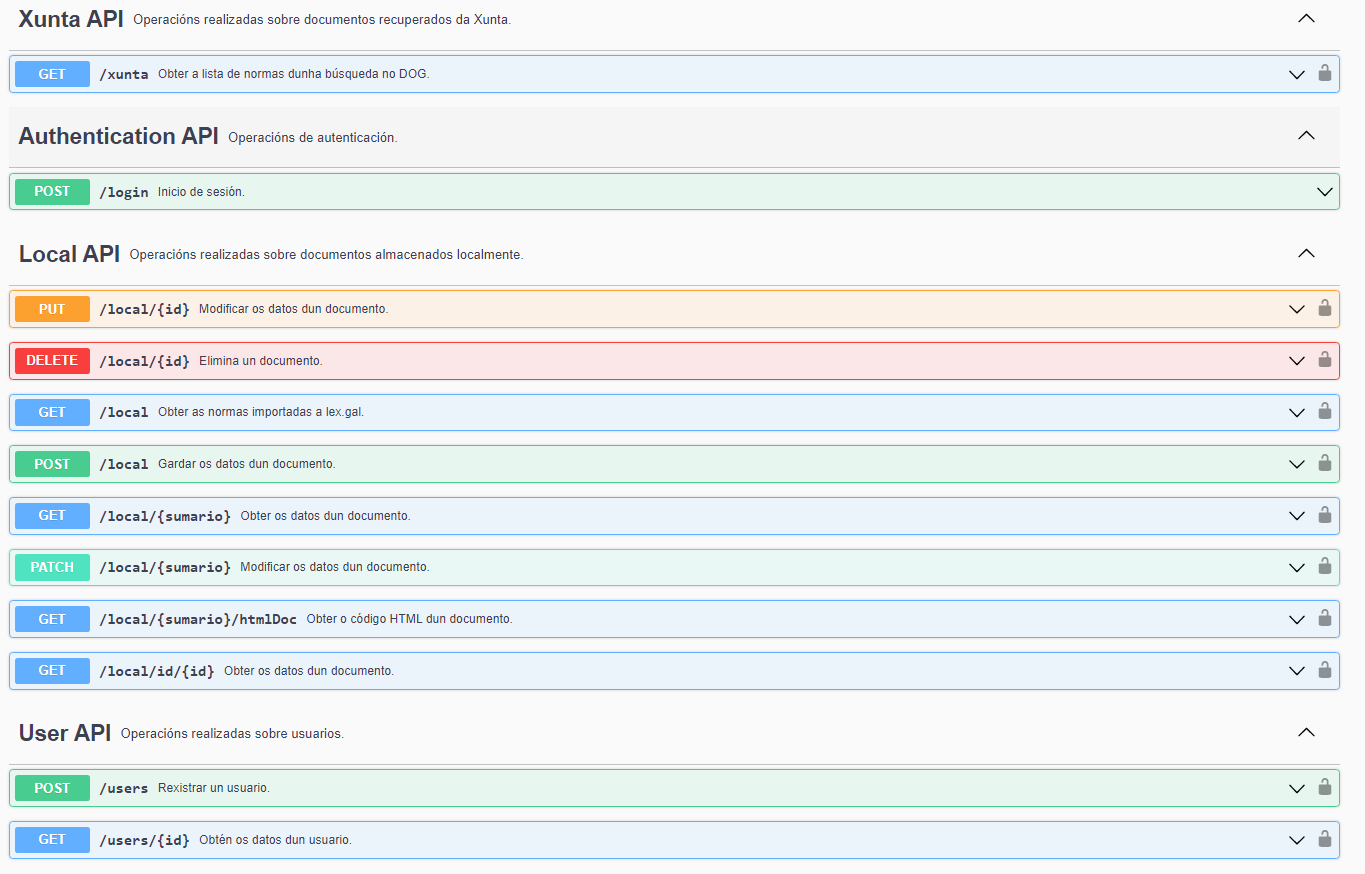
\includegraphics[width=12cm]{figuras/diseño/APIServidor.PNG}}
\caption{API del servidor.}
\label{enlaceAPIServidor}
\end{figure}

En la \hyperref[enlaceAPIServidor]{Figura 3.3} se pueden observar los distintos servicios en la plataforma de Swagger.